\chapter{Antiferromagnetism}
	
	\section{Mott transition}

		Consider a system with $N$ Na atoms, at $T=0$. The electronic configuration of the Na atoms is [Ne]3s$^1$. The Hamiltonian contains a term
		\be \mc H_\text{band} = \varepsilon_\text{3s} \sum_{\vb* j \sigma} n_{\vb* j \sigma} - t_\text{3s} \sum_{\langle \vb* j \vb* l \rangle} \sum_\sigma [c^\dagger_{\vb* j \sigma} c_{\vb* l \sigma} + c^\dagger_{\vb* l \sigma} c_{\vb* j \sigma}] \ee
		with $n_{\vb* j \sigma} = c^\dagger_{\vb* j \sigma} c_{\vb* j \sigma}$ and $t_\text{3s}>0$.	The band structure of this system is given in  \autoref{fig:tbBandStructureNa}. Only the 3s band is half-filled, thus Na is expected to be metal according to band theory, for any lattice constants, since even the 3s band in narrowing as one increases $a$, it remains half-filled. This leads to an absurdity since for a large $a$, \electron would remain on site.

		\begin{figure}[h!]
			\centering
			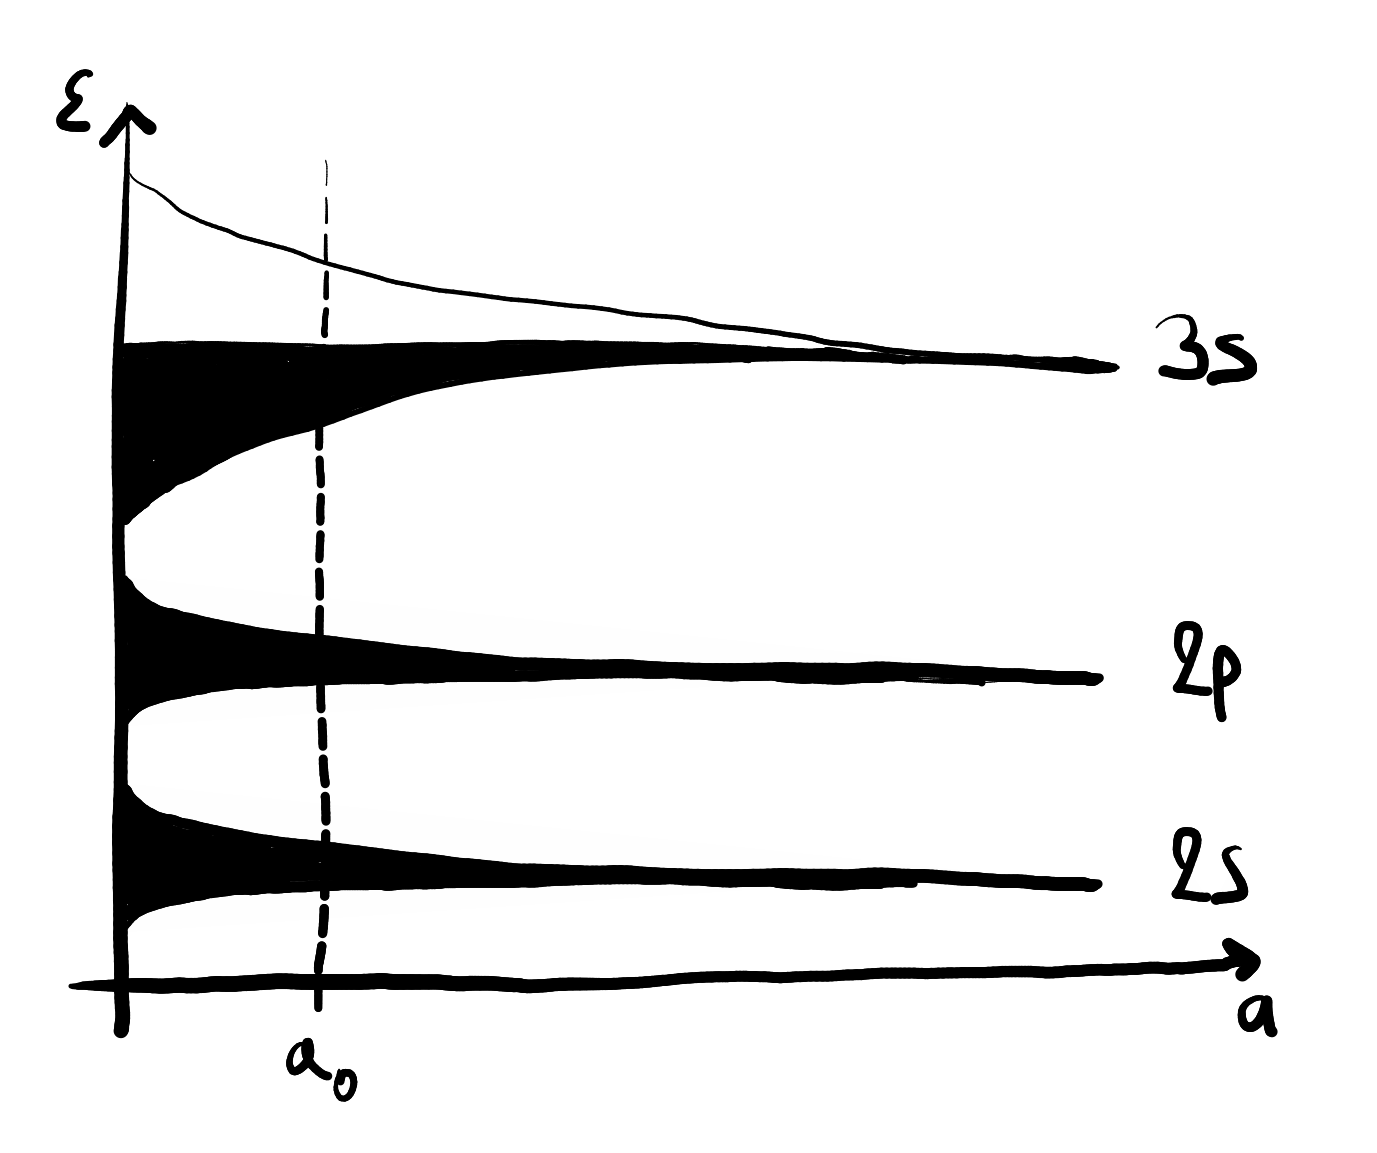
\includegraphics[scale=0.2]{graphs/tbBandStructureNa.png}
			\caption{Tight-binding band structure of Na.}
			\label{fig:tbBandStructureNa}
		\end{figure}

		For electrical conduction, \electron should propagate through the lattice inducing charge fluctuations, as shown on  \autoref{fig:hoppingNaElectron}. Each \electron in a 3s band has energy $\varepsilon_\text{3s}$. If two share the same atomic shell, a repulsion appears leading to the Coulomb energy
		\be U_\text{3s} = \int \dd \vb* r_1 \dd \vb* r_2\ \abs{\phi(\vb* r_1)}^2 \frac{e^2}{\abs{\vb* r_1 - \vb* r_2}} \abs{\phi(\vb* r_2)}^2 \ee

		\begin{figure}[h!]
			\centering
			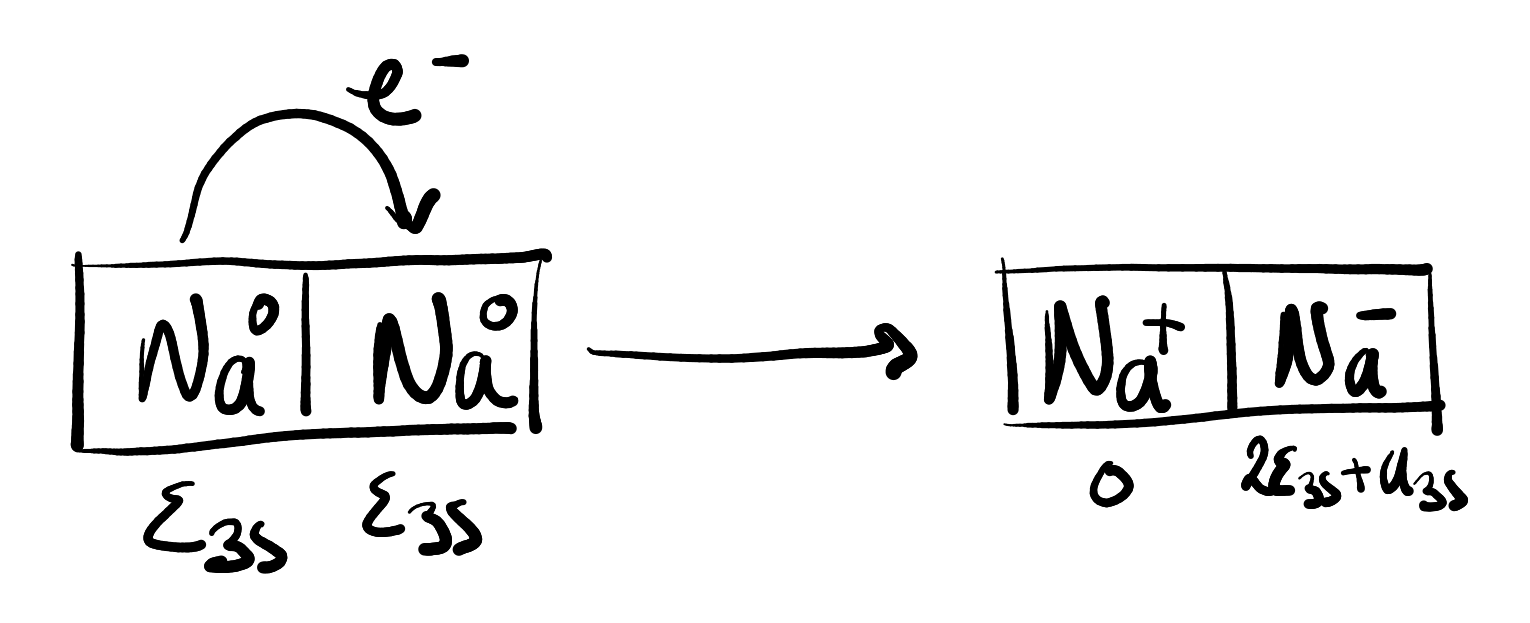
\includegraphics[scale=0.2]{graphs/hoppingNaElectron.png}
			\caption{Charge fluctuation showing an \electron hopping to form an higher energetic doubly-occupied site.}
			\label{fig:hoppingNaElectron}
		\end{figure}

		This process usually costs a lot of energy so it does not want to happen. This suppresses charge fluctuations that are necessary for metallic conduction, leading to a metallic-insulator transition for $a$ above some critical value.

		The total Hamiltonian is thus $\mc H = \mc H_\text{band} + \mc H_\text{Coulomb}$ with
		\be \mc H_\text{Coulomb} = U_\text{3s} \sum_{\vb* j} n_{\vb* j \uparrow} n_{\vb* j \downarrow} \ee
		The kinetic term $\mc H_\text{band}$ can be written making use of the Bloch operators
		\be \mc H_\text{band} = \sum_{\vb* k \sigma} \varepsilon_{\vb* k} c^\dagger_{\vb* k \sigma} c_{\vb* k \sigma} \ee
		whose ground state is the metallic Fermi sea corresponding to the uncorrelated ground state
		\be \ket{\text{FS}} = \prod_{\vb* k}^{\varepsilon_{\vb* k}<\varepsilon_\text{3s}} c^\dagger_{\vb* k \uparrow} c^\dagger_{\vb* k \downarrow} \ket 0 \ee
		remembering that $ c^\dagger_{\vb* k \sigma} = \frac{1}{\sqrt N} \sum_{\vb* j} e^{i \vb* k \cdot \vb* j} c^\dagger_{\vb* j \sigma}$. This leads the the expectation value
		\be \frac{1}{N} \ev{\mc H_\text{3s}}{\text{FS}} = \varepsilon_\text{3s} - \alpha t_\text{3s} + \frac{U_\text{3s}}{4} \ee
		Therefore, increasing $a$ makes $t_\text{3s}$ fall exponentially, leading to $U_\text{3s}/t_\text{3s}$ passing through the critical value $4\alpha$, indicating that the Coulomb energy cost of charge fluctuation exceeds the kinetic energy gain for occupying the lower half of a band. Hence the formation of the band --- an itinerant ground state --- is no longer favorable, leading to a localization of each \electron alone on a single site. To sum up, if $U_\text{3s}/t_\text{3s}< 4\alpha$, the uncorrelated $\ket{\text{FS}}$ is the ground state, and if $U_\text{3s}/t_\text{3s}>4\alpha$, the system is an array of neutral Na atoms. The transition is shown on  \autoref{fig:transitionNa}.
		
		\begin{figure}[h!]
			\centering
			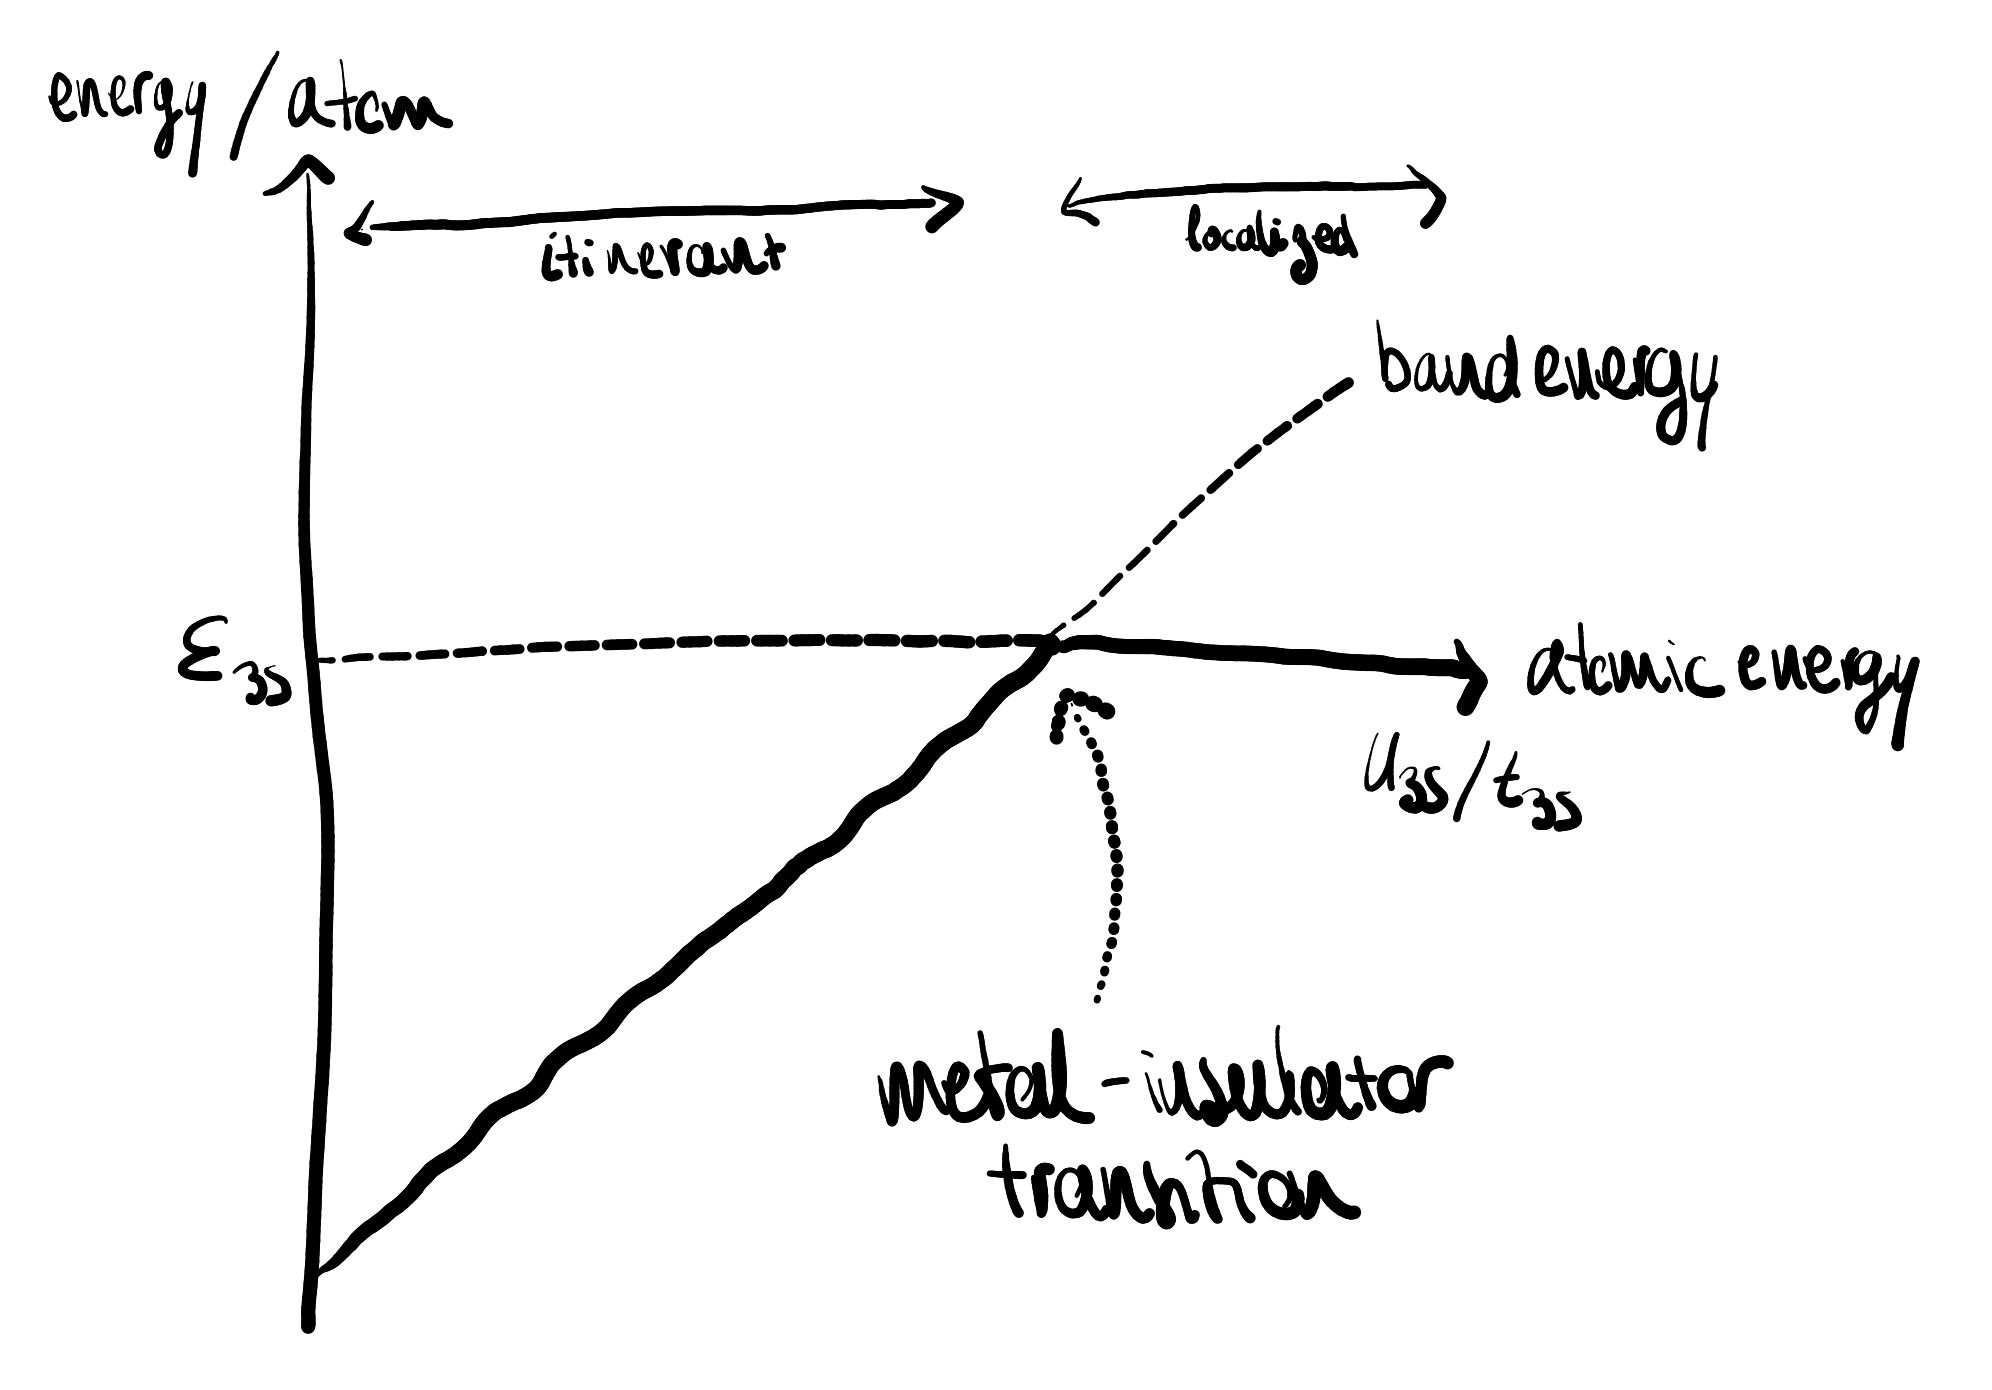
\includegraphics[scale=0.15]{graphs/transitionNa.png}
			\caption{Naive Mott transition showing the metal-insulator transition for the Na system.}
			\label{fig:transitionNa}
		\end{figure}

		Thereby, the insulating system is highly correlated, since the \electron avoid themselves a lot to minimize the Coulomb interaction. Also, $\ket{\text{FS}}$ is not unique since $2^N$-fold degeneracy in the limit $U_\text{3s}/t_\text{3s}\to \infty$ and should be lifted for any finite value. Finally, Mott insulator just described turn out to be antiferromagnets, especially in the large-$U$ limit where writing its Heisenberg Hamiltonian makes this explicit.

	\section{Mean field approximation}

		Magnetic order arises from the inequivalence between the number of up- and down-spins. For this to be understood introduce the $z$-component of the spin at site $\vb* j$ as
		\be \ev{S_{\vb* j}^z} = \frac{\ev{n_{\vb* j \uparrow}} - \ev{n_{\vb* j \downarrow}}}{2} \ee

		Hence, a magnetically ordered state has $\langle S_{\vb* j}^z \rangle \neq0$ either $\forall \vb* j$ or $\forall \vb* j \in \mc A$ where $\mc A$ describes a sublattice of the sites. Since Hubbard Hamiltonian
		\be \mc H = -t \sum_{\langle \vb* j \vb* l \rangle} \sum_\sigma [c^\dagger_{\vb* j \sigma} c_{\vb* l \sigma} + c^\dagger_{\vb* l \sigma} c_{\vb* j \sigma}] + U \sum_{\vb* j} n_{\vb* j \uparrow} n_{\vb* j \downarrow} \ee 
		has spin-rotational invariance, finding a magnetically ordered ground states underlies a symmetry-breaking. Now, express
		\be \begin{split} n_{\vb* j \uparrow}n_{\vb* j \downarrow} &= [n_{\vb* j \uparrow} - \ev{n_{\vb* j \uparrow}}+\ev{n_{\vb* j \uparrow}}][n_{\vb* j \downarrow} - \ev{n_{\vb* j \downarrow}}+\ev{n_{\vb* j \downarrow}}] \\ &= [n_{\vb* j \uparrow} - \ev{n_{\vb* j \uparrow}}]\ev{n_{\vb* j \uparrow}} + [n_{\vb* j \downarrow} - \ev{n_{\vb* j \downarrow}}]\ev{n_{\vb* j \downarrow}} \\ &+ \ev{n_{\vb* j \uparrow}}\ev{n_{\vb* j \downarrow}} + [n_{\vb* j \uparrow} - \ev{n_{\vb* j \uparrow}}][n_{\vb* j \downarrow} - \ev{n_{\vb* j \downarrow}}] \end{split} \ee
		Mean field approximation consists in considering the fluctuations of the spins around their mean value as negligible, hence neglect the last term, leading to
		\be n_{\vb* j \uparrow}n_{\vb* j \downarrow} \sim n_{\vb* j \uparrow}\ev{n_{\vb* j \uparrow}} + n_{\vb* j \downarrow}\ev{n_{\vb* j \downarrow}} - \ev{n_{\vb* j \uparrow}}\ev{n_{\vb* j \downarrow}} \label{eq:decoupling} \ee
		and thus writing $n_{\vb* j} = n_{\vb* j \uparrow} + n_{\vb* j \downarrow}$ gives
		\be 2 n_{\vb* j \uparrow}n_{\vb* j \downarrow} \sim n_{\vb* j}\ev{n_{\vb* j}} - 4 S_{\vb* j}^z \ev{S_{\vb* j}^z} - \frac{\ev{n_{\vb* j}}^2}{2} + 2 \ev{S_{\vb* j}^z}^2  \ee
		However, the Hubbard Hamiltonian being isotropic, one has to be careful to not prefer one particular orientation of the spin and write the complete Hartree-Fock approximation, but one is not going to seek into cumbersome derivations rather fix the $z$-axis. Finally writing this decoupled scheme, neglecting local charge deviation $\ev{\delta n_{\vb* j}} = 0$, one finds
		\be U \sum_{\vb* j} n_{\vb* j \uparrow} n_{\vb* j \downarrow} \sim -2U \sum_{\vb* j} \vb* S_{\vb* j} \ev{\vb* S_{\vb* j}} +  U \sum_{\vb* j} \ev{\vb* S_{\vb* j}^2} + \frac{LUn^2}{4} \ee
		with $n = N/L$.

	\section{Stoner model}

		The goal is to find a criterion for the Hubbard model to be ferromagnetic. Into a uniform magnetic field, express
		\be \mc H = \sum_{\vb* k \sigma} \epsilon_{\vb* k \sigma} n_{\vb* k \sigma} + U \sum_{\vb* j} n_{\vb* j \uparrow}n_{\vb* j \downarrow} - \frac{g\mu_\text{B} H}{2} \sum_{\vb* j} [n_{\vb* j \uparrow}-n_{\vb* j \downarrow}] \ee
		leading to a uniform spin polarization $m$ allowing to write
		\be \ev{n_{\vb* j \uparrow}} = \frac{n}{2} + m \qq{and} \ev{n_{\vb* j \downarrow}} = \frac{n}{2} - m \ee
		The mean field decoupling \eqref{eq:decoupling} helping, one finds the total energy density
		\be \mc E(m)= \int_B^{\mu_\uparrow} \dd \varepsilon \ \rho(\varepsilon)\varepsilon + \int_B^{\mu_\downarrow} \dd \varepsilon \ \rho(\varepsilon)\varepsilon + U\left[\frac{n^2}{2} - m^2 \right] - g\mu_\text{B} Hm \ee
		where $B$ is the bottom energy of the band as presented on  \autoref{fig:stonerBand}, and with $\mu_\sigma$ such that $n_\sigma = \int_B^{\mu_\sigma} \dd \varepsilon \ \rho(\varepsilon)$. Now, try to find the energy change induced by the polarization
		\be \begin{split} \Delta \mc E(m) &= \mc E(m) - \mc E(0) \\ &= \int_{\mu_0}^{\mu_\uparrow} \dd \varepsilon \ \rho(\varepsilon)\varepsilon - \int_{\mu_0}^{\mu_\downarrow} \dd \varepsilon \ \rho(\varepsilon)\varepsilon - Um^2 - g\mu_\text{B} Hm \end{split} \ee 
		with $\mu_0$ the chemical potential for $H=0$.

		\begin{figure}[h!]
			\centering
			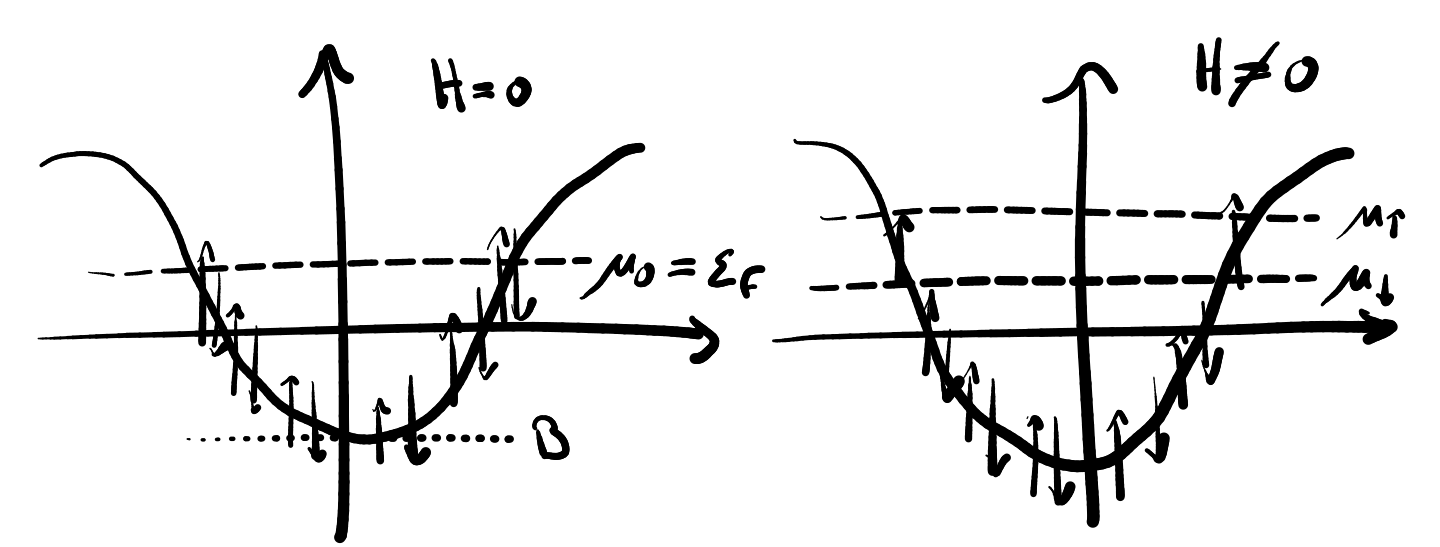
\includegraphics[scale=0.2]{graphs/stonerBand.png}
			\caption{Chemical potentials with and without magnetic field.}
			\label{fig:stonerBand}
		\end{figure}

		Increasing $U$ starting from $0$ yields a $T=0$ paramagnetic-ferroma-\\gnetic transition. Consider it to be of second order. Then, $m$ is continuously induced by $H$. For $H\ll 1$, one can replace $\rho(\varepsilon) \simeq \rho(\varepsilon_\text{F})$ and at second order
		\be \Delta \mc E(m) = \frac{m^2}{\rho(\varepsilon_\text{F})} - Um^2 - g\mu_\text{B}Hm \ee
		Further minimizing with respect to $m$ yields the susceptibility being
		\be \chi = \frac{m g\mu_\text{B}}{H} = \frac{(g\mu_\text{B})^2}{2} \frac{\rho(\varepsilon_\text{F})}{1-U\rho(\varepsilon_\text{F})} \ee
		which diverges for the critical
		\be U_\text{crit} \rho(\varepsilon_\text{F}) = 1 \label{eq:stoner} \ee
		This is the Stoner criterion, which implies that approaching $U_\text{crit}$ from below yields a divergence of $\chi$ and thus an instability of the symmetric paramagnetic ground state, falling into a ferromagnetic ordering. Finally, this means that as long as $\rho(\varepsilon_\text{F}) \neq 0$, ferromagnetism is ensured by the Stoner criterion at sufficiently large $U$. The problem is that near half-filling, the Hubbard model prefers antiferromagnetism. This leads to the generalized Stoner model.

	\section{Generalized Stoner model}

		The instability of the Hubbard model must take the form of a divergent response to an external magnetic field with wavevector $\vb* q$. The full Hamiltonian is 
		\be \mc H = \mc H_\text{band} + \mc H_U + \mc H_\text{field} \ee
		The coupling of the spins to the field is
		\be \mc H_\text{field} = - \int \dd \vb* r \ \vb* H(\vb* r) \cdot \vb* M(\vb* r) = -g\mu_\text{B} \int \dd \vb* r \ \vb* H(\vb* r) \cdot \vb* S(\vb* r) \ee
		where $\vb* M(\vb* r)$ is the density of magnetic moment and $\vb* S(\vb* r) = \sum_j \delta(\vb* r - \vb* r_j) \vb* S_j$ the density of spin. Go to the Fourier space as
		\be \vb* S(\vb* q) = \int \dd \vb* r \ e^{-i\vb* q \cdot \vb* r} \vb* S(\vb* r) = \sum_j e^{-i\vb* q \cdot \vb* r_j} \vb* S_j \ee
		Looking for a period magnetic field $\vb* H(\vb* r) = \vb* H_{\vb* q} \cos \vb* q \cdot \vb* r$, and knowing the Hamiltonian is spin-rotationally invariant, choose the $x$-direction and find
		\be \begin{split} \mc H_\text{field} &= -g\mu_\text{B} \sum_j \vb* H(\vb* r_j) \cdot \vb* S_j \\ &= -g\mu_\text{B}  \sum_j H^x S_j^x \frac{e^{i\vb* q \cdot \vb* r_j} + e^{-i\vb* q \cdot \vb* r_j}}{2} \\ &= -\frac{g\mu_\text{B} H^x}{2}[S^x(\vb* q) + S^x(-\vb* q)] \end{split} \label{eq:hField} \ee
		Now, writing 
		\be \begin{split} n_{\vb* j \uparrow}n_{\vb* j \downarrow} &= c^\dagger_{\vb* j \uparrow}c_{\vb* j \uparrow}c^\dagger_{\vb* j \downarrow}c_{\vb* j \downarrow} = n_{\vb* j \uparrow} - c^\dagger_{\vb* j \uparrow}c_{\vb* j \downarrow}c^\dagger_{\vb* j \downarrow}c_{\vb* j \uparrow} \\ &= n_{\vb* j \uparrow} - S^+_{\vb* j} S^-_{\vb* j} \\ \qq{and} n_{\vb* j \uparrow}n_{\vb* j \downarrow} &= n_{\vb* j \downarrow} - S^-_{\vb* j} S^+_{\vb* j} \end{split} \ee
		one arrives at the expression
		\be \mc H_U = U \sum_{\vb* j} n_{\vb* j \uparrow}n_{\vb* j \downarrow} = \frac{NU}{2} - U \sum_{\vb* j} [(S^x_{\vb* j})^2 + (S^y_{\vb* j})^2] \ee
		Then decoupling like $(S^x_{\vb* j})^2 \sim 2 S^x_{\vb* j} \langle S^x_{\vb* j}\rangle - \langle S^x_{\vb* j}\rangle^2$ and assuming that the only non-vanishing average is due to the spin density wave induced by the external magnetic field, \emph{ie} neglecting the $y$ component, as long as writing $\langle S^x_{\vb* j}\rangle = \mc S \cos  \vb* q \cdot \vb* j$, one finds
		\be \mc H_U = -U \mc S[S^x(\vb* q) + S^x(-\vb* q)] \ee
		Write the term
		\be \mc H' = - \left[\frac{g\mu_\text{B} H^x}{2} + U\mc S \right][S^x(\vb* q) + S^x(-\vb* q)] \ee
		Treat now the spin density as $\mc S\ll 1$. Then $\mc H'$ is to be considered as a perturbation of $\mc H_\text{band}$ whose ground state is the Fermi sea $\ket{\text{FS}}$. Via first-order perturbation theory
		\be \begin{split} \ket \psi = \ket{\text{FS}} - &\left[\frac{g\mu_\text{B} H^x}{2} + U\mc S \right] \\ &\cdot \sum_{\vb* p \sigma} \left[ \frac{c^\dagger_{\vb* p + \vb* q, \sigma} c_{\vb* p, -\sigma}}{\varepsilon_{\vb* p} - \varepsilon_{\vb*p + \vb* q}} + \frac{c^\dagger_{\vb* p - \vb* q, \sigma} c_{\vb* p, -\sigma}}{\varepsilon_{\vb* p} - \varepsilon_{\vb*p - \vb* q}} \right] \ket{\text{FS}} \end{split} \ee
		having used the $S^x(\vb* q) = \frac{1}{2} \sum_{\vb* p \sigma} c^\dagger_{\vb* p + \vb* q, \sigma} c_{\vb* p, -\sigma}$. Now computing at first order and assuming $\vb* q \neq 0$
		\be \begin{split} \frac{\ev{c^\dagger_{\vb* p + \vb* q, \sigma} c_{\vb* p, -\sigma}}{\psi}}{\frac{g\mu_\text{B} H^x}{2} + U\mc S} = - \sum_{\vb* k \sigma'} \bra{\text{FS}} &\left[ \cancel{\frac{c^\dagger_{\vb* p + \vb* q, \sigma} c_{\vb* p, -\sigma} c^\dagger_{\vb* k + \vb* q, \sigma'} c_{\vb* k, -\sigma'}}{\varepsilon_{\vb* k} - \varepsilon_{\vb*k + \vb* q}}} \right. \\ &+ \frac{c^\dagger_{\vb* p + \vb* q, \sigma} c_{\vb* p, -\sigma} c^\dagger_{\vb* k - \vb* q, \sigma'} c_{\vb* k, -\sigma'}}{\varepsilon_{\vb* k} - \varepsilon_{\vb*k - \vb* q}} \\ &+ \frac{c^\dagger_{\vb* k, -\sigma'} c_{\vb* k + \vb* q, \sigma'} c^\dagger_{\vb* p + \vb* q, \sigma} c_{\vb* p, -\sigma}}{\varepsilon_{\vb* k} - \varepsilon_{\vb*k + \vb* q}} \\ &+ \left. \cancel{\frac{c^\dagger_{\vb* k, -\sigma'} c_{\vb* k - \vb* q, \sigma'} c^\dagger_{\vb* p + \vb* q, \sigma} c_{\vb* p, -\sigma}}{\varepsilon_{\vb* k} - \varepsilon_{\vb*k - \vb* q}}} \right] \ket{\text{FS}} \end{split} \label{eq:bigMessEv} \ee
		where the cancellation comes from the impossibility to recover the Fermi sea without taking $\vb* q=0$. Introducing the occupying function as the Fermi-Dirac distribution at $T=0$
		\be f_{\vb* p} = \Theta (\varepsilon_\text{F} - \varepsilon_{\vb* p}) = \ev{c^\dagger_{\vb* p \sigma} c_{\vb* p \sigma}}{\text{FS}} \ee
		the first non-vanishing term in \eqref{eq:bigMessEv} imposes $\vb* k = \vb* p + \vb* q$ and the second one $\vb* k = \vb* p$. This yields, using the anti-commutation relations
		\be \begin{split} \frac{\ev{c^\dagger_{\vb* p + \vb* q, \sigma} c_{\vb* p, -\sigma}}{\psi}}{\frac{g\mu_\text{B} H^x}{2} + U\mc S} &= - \frac{f_{\vb* p}(1- f_{\vb* p + \vb* q}) - f_{\vb* p + \vb* q}(1-f_{\vb* p})}{\varepsilon_{\vb* p} - \varepsilon_{\vb*p + \vb* q}} \\ &= \frac{f_{\vb* p} - f_{\vb* p + \vb* q}}{\varepsilon_{\vb*p + \vb* q} -\varepsilon_{\vb* p}} \end{split} \ee
		Hence, introducing 
		\be \chi^{(0)}(\vb* q) = \sum_{\vb* p} \frac{f_{\vb* p} - f_{\vb* p + \vb* q}}{\varepsilon_{\vb*p + \vb* q} -\varepsilon_{\vb* p}} \ee
		one gets
		\be \mc S = \ev{S^x(\vb* q)}{\psi} = \left[\frac{g\mu_\text{B} H^x}{2} + U\mc S \right] \chi^{(0)}(\vb* q) \ee 
		and rearranging the terms of the auto-coherent equation for the spin density
		\be \implies \mc S = \frac{g\mu_\text{B}H^x}{2} \frac{\chi^{(0)}(\vb* q)}{1- U \chi^{(0)}(\vb* q)} \label{eq:spinDensityGen} \ee
		which gives the generalized $\vb* q$-dependent static susceptibility 
		\be \chi(\vb* q) = (g\mu_\text{B})^2 \frac{\chi^{(0)}(\vb* q)}{1- U \chi^{(0)}(\vb* q)} \ee
		making use of \eqref{eq:hField} and minimizing $\ev{\mc H_\text{field}}{\psi}$ with respect to $H^x$ then inserting \eqref{eq:spinDensityGen} and recovering the magnetization density.	The generalized Stoner criterion then reads
		\be U^{\vb* q}_\text{crit} \chi^{(0)}(\vb* q) = 1 \ee
		To recover the Stoner criterion \eqref{eq:stoner}, take the $\vb* q \to 0$ limit. Then 
		\be \begin{split} f_{\vb* p} - f_{\vb* p + \vb* q} &\simeq -\pdv{f}{\varepsilon} \pdv{\varepsilon}{\vb* p} \cdot \vb* q \\ \qq{and} \varepsilon_{\vb*p + \vb* q} -\varepsilon_{\vb* p} &\simeq \pdv{\varepsilon}{\vb* p} \cdot \vb* q \end{split} \ee
		which implies 
		\be \chi^{(0)}(\vb* q) \simeq -\int \dd \varepsilon \ \rho(\varepsilon) \pdv{f}{\varepsilon} = \rho(\varepsilon_\text{F}) \ee
		since at $T=0$ one has $\pdv{f}{\varepsilon} = -\delta(\varepsilon - \varepsilon_\text{F})$. Therefore, at arbitrary band-filling, the system becomes unstable against the formation of a spin density wave with arbitrary $\vb* q$ if $U$ is large enough. Only the instability occurring at the lowest $U_\text{crit} = \min_{\vb* q} U^{\vb* q}_\text{crit}$ happens. This peaks out a certain $\vb* q_0$ for the spin density wave, which depends on the band-filling. Increasing further $U$ beyond its critical value leads to a saturation of the amplitude of the wave, yielding sometimes a phase transition to another magnetic ordering.

		Taking a $D$-dimensional cubic lattice, the dispersion relation reads
		\be \varepsilon(\vb* k) = -2t \sum_{i=1}^D \cos k_i \ee
		and it satisfies the perfect nesting condition $ \varepsilon(\vb* k + \vb* Q) =  -\varepsilon(\vb* k) \ \forall \vb* k$, where $\vb* Q = (\pi,\dotsc, \pi)$ is the spanning-vector. At half-filling, $\varepsilon_\text{F} = 0$, and at $T=0$ one has
		\be \chi^{(0)}(\vb* Q) = \int_0^{w/2} \dd \varepsilon \ \frac{\rho(\varepsilon)}{2\varepsilon} \ee
		with $w$ the bandwidth. Unless $\rho(\varepsilon) \to 0$ as $\varepsilon \to 0$, $\chi^{(0)}(\vb* Q)$ diverges logarithmically. Hence $U_\text{crit}^{\vb* Q}=0$ that is, for half-filled bands with the perfect nesting property, an arbitrary small $U>0$ causes a transition to a two-sublattice antiferromagnetic state. In fact, it can be shown by approximating the Fermi-Dirac distribution correctly, one has
		\be \chi^{(0)}(\vb* Q, T) \sim \frac{1}{t} \ln \frac{t}{2k_\text{B} T} \qq{and} \chi^{(0)}(0, T) \sim \frac{1}{t} \ln^2 \frac{t}{2k_\text{B} T} \ee
		which means that the antiferromagnetic instability is stronger than the ferromagnetic one, since for $T\to 0$, the response diverges faster for $\vb* q = \vb* Q$ than for $\vb* q = 0$.

		Finally, one can show that the antiferromagnetic state is insulating, meaning that the metal-insulator transition occurs at $U=0$ here. This comes from writing the Hamiltonian in mean field approximation
		\be \mc H_\text{SDW} = \mc H_\text{band} + U\sum_{\vb* j \sigma} n_{\vb* j \sigma}  \ev{n_{\vb* j, -\sigma}} - U \sum_{\vb* j} \ev{n_{\vb* j \uparrow}} \ev{n_{\vb* j \downarrow}} \ee
		and diagonalizing it to obtain, assuming perfect nesting
		\be \lambda^\pm(\vb* k) = \frac{Un}{2} \pm \sqrt{\varepsilon^2_{\vb* k} + U^2 m^2} \ee
		giving a band gap of $2Um$.